\documentclass[11pt]{article}
\usepackage[T1]{fontenc}
\usepackage[scaled]{uarial}
\usepackage{graphicx}
\renewcommand*\familydefault{\sfdefault} 
\usepackage[margin=1in]{geometry}
\usepackage{setspace}
\usepackage{color}

\definecolor{OptColor}{RGB}{157, 47, 47}
\definecolor{PesColor}{RGB}{208, 98, 98}
\definecolor{CauColor}{RGB}{47, 87, 157}
\definecolor{ConColor}{RGB}{98, 138, 208}
\definecolor{NeuColor}{RGB}{102, 102, 102}


\newcommand{\opt}[1]{\textcolor{OptColor}{#1}}
\newcommand{\pes}[1]{\textcolor{PesColor}{#1}}
\newcommand{\cau}[1]{\textcolor{CauColor}{#1}}
\newcommand{\con}[1]{\textcolor{ConColor}{#1}}
\newcommand{\neu}[1]{\textcolor{NeuColor}{#1}}


\begin{document}
\thispagestyle{empty}
\begin{center} \textbf{EXPLAINING AWAY IN SEMANTIC ADAPTATION}  \\
\end{center}
\vspace{-1em}
\noindent \textbf{Keywords}: explaining away, adaptation, semantics, pragmatics, uncertainty expressions


\noindent Speakers exhibit considerable production variability at all levels of linguistic representation. Listeners deal with such variability by adapting to it and updating expectations [1-5]. This includes adaptation to uncertainty expressions: In interaction, listeners learn speaker-specific semantic representations and speaker preferences for different uncertainty expressions such as \textit{might} and \textit{probably} after exposure to speakers who use these expressions differently [5,6]. This behavior is predicted by a model based on Bayesian belief updating [5], which suggests that listeners track utterance-event likelihood pairs and refine expectations based on this statistical input. However, it remains an open question whether this learning is purely \textbf{associative}, i.e., listeners track the associations between utterances and event likelihoods independent of other contextual factors, or if listeners engage in a more elaborate learning process and \textbf{explain away} unexpected behavior if they are presented with a likely cause [7].  We build upon findings that speakers use uncertainty expressions differently depending on contextual factors [8,9] and investigate whether manipulation of one contextual factor, namely information about a speaker's mood, affects the adaptation behavior. According to an {associative} account, we expect no effect of mood on the adaptation behavior whereas an {explaining away} account would predict less adaptation if the speaker behavior matches expected language use for the mood. 

\noindent \textbf{Exp.~1 (norming)} tested whether mood affects expectations about the use of \textit{might} and \textit{probably}.  53 MTurk participants saw 36 images of an airline representative interacting with a customer, along with a seat map that illustrated the likelihood of the customer being randomly assigned their desired seat (see Fig.~1). Participants in the \textit{\opt{optimist}} and \textit{\pes{pessimist}} conditions saw a representative who was in a good or bad mood, respectively; participants in the \textit{\neu{neutral}} condition did not receive information about the mood. The probability of receiving the desired seat ranged from  0\% to 100\%. Participants were asked to rate likely responses to the customer's request by distributing 100 points across three items, ``You'll probably get one,'' ``You might get one,'' and a \textit{something else} option. As Fig.~2 shows, \textit{probably} was rated higher than \textit{might} for a greater range of likelihoods in the \textit{\opt{optimist}} condition than in the \textit{\pes{pessimist}} condition. Like [4,5], we quantified this difference by  computing the area under the curve (AUC) for each participant and expression. We found that the average difference between the AUC of \textit{might} and \textit{probably} is smaller in the \textit{\opt{optimist}} cond. than in the \textit{\pes{pessimist}} cond. ($t(34)=-2.51$, $p < 0.05$), suggesting that mood affects expectations about the use of \textit{might} and \textit{probably}. 

\noindent \textbf{Exp.~2 (explaining away)} tested whether information about the speaker's mood affects adaptation. 268 MTurk participants saw 13 exposure trials (5 critical, 8 fillers) followed by 36 test trials. Exposure trials showed an image of an airline representative describing a seat map with window and aisle seats (critical trials: 60\% window seats). There were 4 conditions--\textit{\opt{OPTimist}}, \textit{\con{CONfident}}, \textit{\pes{PESsimist}}, \textit{\cau{CAUtious}}--where participants in \opt{OPT} and \con{CON} listened to a speaker using \textit{probably} at 60\%, and participants in \pes{PES} and \cau{CAU} listened to a speaker using \textit{might} at 60\%. Fillers were intended to boost trust in the speaker: on 5 trials, the speaker described a typical (25\% or 90\%) probability with the respective other uncertainty expression. On other fillers, the speaker said of a 100\% window seat probability ``You'll get one.'' Additionally, for the exposure in \opt{OPT} and \pes{PES}, participants were told the speaker was happy or angry, respectively. The test trials were the same as in Exp.~1, except that before the test trials, participants were told the speaker was experiencing a normal day. Fig.~3 shows the ratings from this study. We found that the average difference between the AUC of \textit{might} and \textit{probably} is smaller in \con{CON} than in \cau{CAU} ($t(133)=-5.1755$, $p < 0.001$), replicating the adaptation effect [5]. Further, we found that the average difference between the AUC of \textit{might} and \textit{probably} is smaller in \pes{PES} than in \cau{CAU} ($t(135)=-2.38$, $p < 0.05$) and qualitatively smaller in \con{CON} than in \opt{OPT}, suggesting that listeners adapted less when provided with a likely explanation for the speaker's language use.

\noindent \textbf{Conclusion}: Our experiments provide evidence for listeners incorporating contextual cues when learning speaker-specific expectations about language use in accordance with an explaining away account.

\hspace{0.06\textwidth}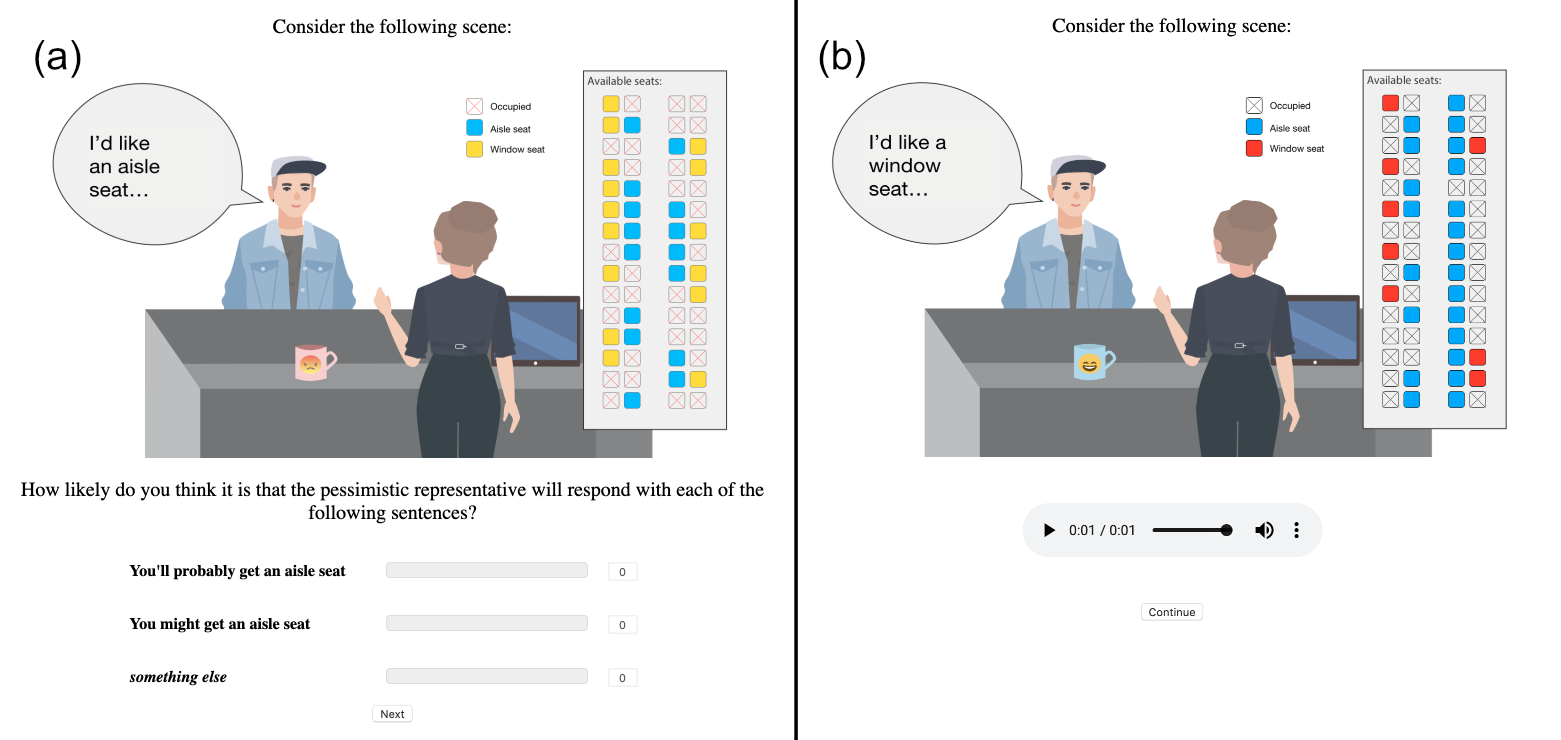
\includegraphics[width=0.8\textwidth]{./plots/example-trial.png}\\
{\small Figure 1: (a) Example trial from Exp.~1. (b) Example exposure trial from Exp.~2.}

\vspace{0.4em}
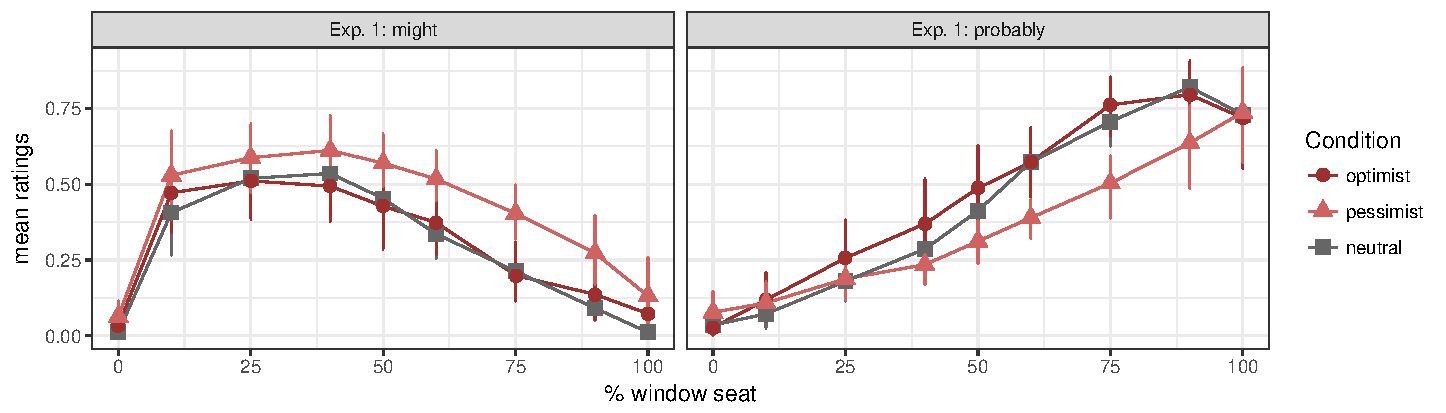
\includegraphics[width=\textwidth]{./plots/norming.pdf}\\
{\small Figure 2: Mean ratings for utterances with \textit{some} and \textit{probably} for the three conditions in the norming experiment (Exp.~1). Error bars indicate bootstrapped 95\% confidence intervals.}

\vspace{0.4em}
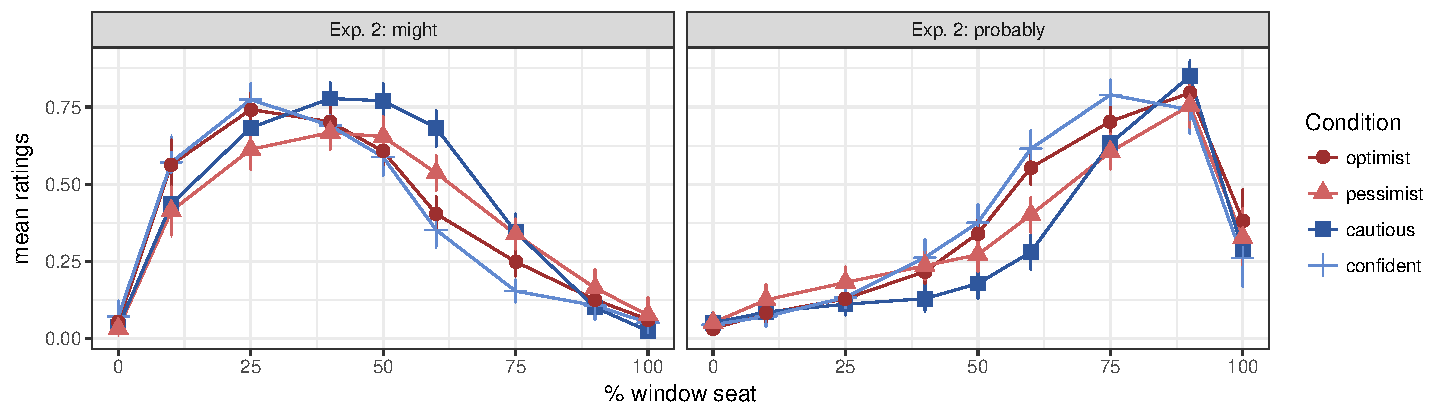
\includegraphics[width=\textwidth]{./plots/exp.pdf}\\
{\small Figure 3: Mean ratings for utterances with \textit{some} and \textit{probably} for the four conditions in the explaining away experiment (Exp.~2). Error bars indicate bootstrapped 95\% confidence intervals. }

\vspace{1em}
\noindent \textbf{References} \\
{\tiny \noindent $[$1$]$ Kleinschmidt, D. \& Jaeger, T.F. (2016). Robust speech perception: Recognize the familiar, generalize to the similar, and adapt to the novel. \textit{Psychological Review}. $[$2$]$ Kamide, Y. (2012). Learning individual talkers' structural preferences. \textit{Cognition}. $[$3$]$~Fine, A.B., Jaeger, T.F., Farmer, T.A. \& Qian, T. (2013). Rapid expectation adaptation during syntactic comprehension. \textit{PLOS ONE}. $[$4$]$ Yildirim, I., Degen, J., Tanenhaus, M.K. \& Jaeger, T.F. (2016). Talker-specificity and adaptation in quantifier interpretation. \textit{Journal of Memory and Language}. $[$5$]$  Schuster, S. \& Degen, J. (under review). I know what you're probably going to say: Listener adaptation to variable use of uncertainty expressions. $[$6$]$  Schuster, S. \& Degen, J. (2019). Speaker-specific adaptation to variable use of uncertainty expressions. $[$7$]$  Kraljic, T., Samuel, A.G., \& Brennan S.E. (2008) First Impressions and Last Resorts: How Listeners adjust to speaker variability. \textit{Psychological Science}. $[$8$]$   Bonnefon, J.F., Feeney, A. \& Villejoubert, G. (2007). When some is actually all: Scalar inferences in face-threatening contexts. \textit{Cognition}. $[$9$]$  Juanchich, M. \& Sirota, M. (2013). Do people really say it is "likely" when they believe it is only "possible"? Effect of politeness on risk communication.
}
\end{document}